\section{Introduction}

    \subparagraph{}Le but de ce {\color{info}7\ieme{} travail} est de proposer une table de vérité d’une fonction 
    logique à 4 entrées (A,B,C,D), en déterminer l’équation logique optimisée via le diagramme de Karnaugh et enfin de 
    simuler le circuit avec le logiciel \textit{LTspice} afin de démontrer l'exactitude des calculs.\\[1.5cm]
    
    \begin{titletbox}{À l'attention du correcteur / correctrice}{warning}
        N'hésitez pas à zoomer sur les schémas du circuit et autres images afin d'y voir plus clair.
    \end{titletbox}

    \section{Table de vérité}

    \subparagraph{}Voici la table de vérité que j'ai choisi (les x symbolisent les don't care) :
        

        \begin{table}[H]
            \centering
            \begin{tabular}{|c|c|c|c|
            >{\columncolor[HTML]{DAE8FC}}c |}
            \hline
            \textbf{A} & \textbf{B} & \textbf{C} & \textbf{D} & \textbf{Y}                                       \\ \hline
            0          & 0          & 0          & 0          & 1                                                \\ \hline
            0          & 0          & 0          & 1          & 0                                                \\ \hline
            0          & 0          & 1          & 0          & \cellcolor[HTML]{CB0000}X                        \\ \hline
            0          & 0          & 1          & 1          & 0                                                \\ \hline
            0          & 1          & 0          & 0          & 0                                                \\ \hline
            0          & 1          & 0          & 1          & \cellcolor[HTML]{CB0000}{\color[HTML]{000000} X} \\ \hline
            0          & 1          & 1          & 0          & 1                                                \\ \hline
            0          & 1          & 1          & 1          & 1                                                \\ \hline
            1          & 0          & 0          & 0          & 0                                                \\ \hline
            1          & 0          & 0          & 1          & \cellcolor[HTML]{CB0000}X                        \\ \hline
            1          & 0          & 1          & 0          & 1                                                \\ \hline
            1          & 0          & 1          & 1          & \cellcolor[HTML]{CB0000}X                        \\ \hline
            1          & 1          & 0          & 0          & 0                                                \\ \hline
            1          & 1          & 0          & 1          & 1                                                \\ \hline
            1          & 1          & 1          & 0          & 0                                                \\ \hline
            1          & 1          & 1          & 1          & 1                                                \\ \hline
            \end{tabular}
            \caption{Table de vérité de la fonction logique}
            \label{tab:truth}
        \end{table}

\newpage
\section{Diagramme de Karnaugh}

    Avec la table de vérité obtenue au point précédent, on construit le diagramme de Karnaugh en respectant certaines règles :
    
        \begin{enumerate}
            \item Chaque "1" doit être encadré au moins une fois.
            \item Chaque rectangle doit être une puissance de 2 (1-2-4-8-16 dans notre cas).
            \item Les rectangles peuvent être d'un bord à un autre.
            \item Les X (don't care) ne sont encadrés que s'ils aident à minimiser l'équation
        \end{enumerate}

        \begin{center}
            \begin{karnaugh-map}[4][4][1][][] % note empty X and Y labels
            \maxterms{1,2,3,4,12,11} % où se trouve les 0
            \minterms{0,7,13,15,9,10} % où se trouve les 1
            \autoterms[X] % tous les autres endroits => X
            \implicant{5}{15} % les lots à prendre (le rouge)
            \implicantedge{0}{0}{8}{8} % les lots à prendre si ça implique les bords (le vert)
            \implicantedge{8}{8}{10}{10} % lot à prendre (le jaune)
            \implicant{8}{9} % lot à prendre (le bleu)
            % note: posistion for start of \draw is (0, Y) where Y is
            % the Y size(number of cells high) in this case Y=4
            \draw[color=black, ultra thin] (0, 4) --
            node [pos=0.8, above right, anchor=south west] {\textcolor{red}{$A B$}} % x0 x1 label
            node [pos=0.6, below left, anchor=north east] {\textcolor{red}{$C D$}} % x2 x3 label
            ++(135:1);
          \end{karnaugh-map}
        \end{center}
        
        
    \subparagraph{}On a donc bien un diagramme respectant les 4 règles énoncées ci-dessus.


\section{Fonction logique optimisée}

    \subparagraph{}Le diagramme nous permet de trouver la fonction suivante : 
         \begin{equation*}
            Y\;=\;\color{mygreen}\overline{A}\overline{B}\overline{D} + \color{cyan} \overline{A}C\overline{D} + 
            \color{kred} BD + \color{kyellow}\overline{B}C\overline{D}
         \end{equation*}

\section{Schéma du circuit}

    \begin{figure}[H]
        \centering
        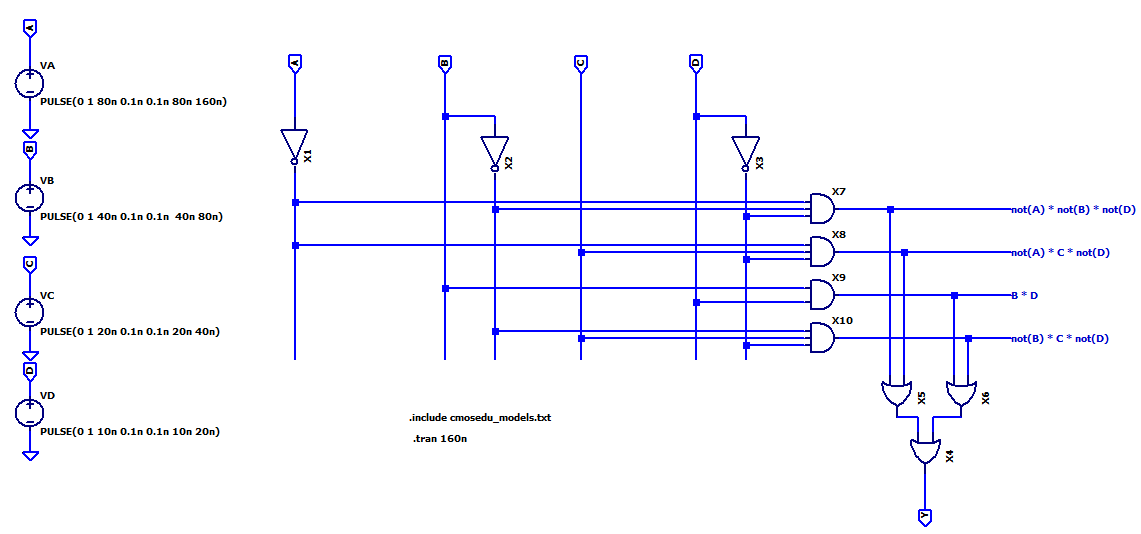
\includegraphics[width=\textwidth]{../pictures/circuit.PNG}
        \caption{Schéma du circuit}
        \label{fig:circuit}
    \end{figure}
    
    
\section{Simulation en parcourant les 16 états}

    \subparagraph{}J'obtiens la simulation suivante :
        
        \begin{figure}[H]
            \centering
            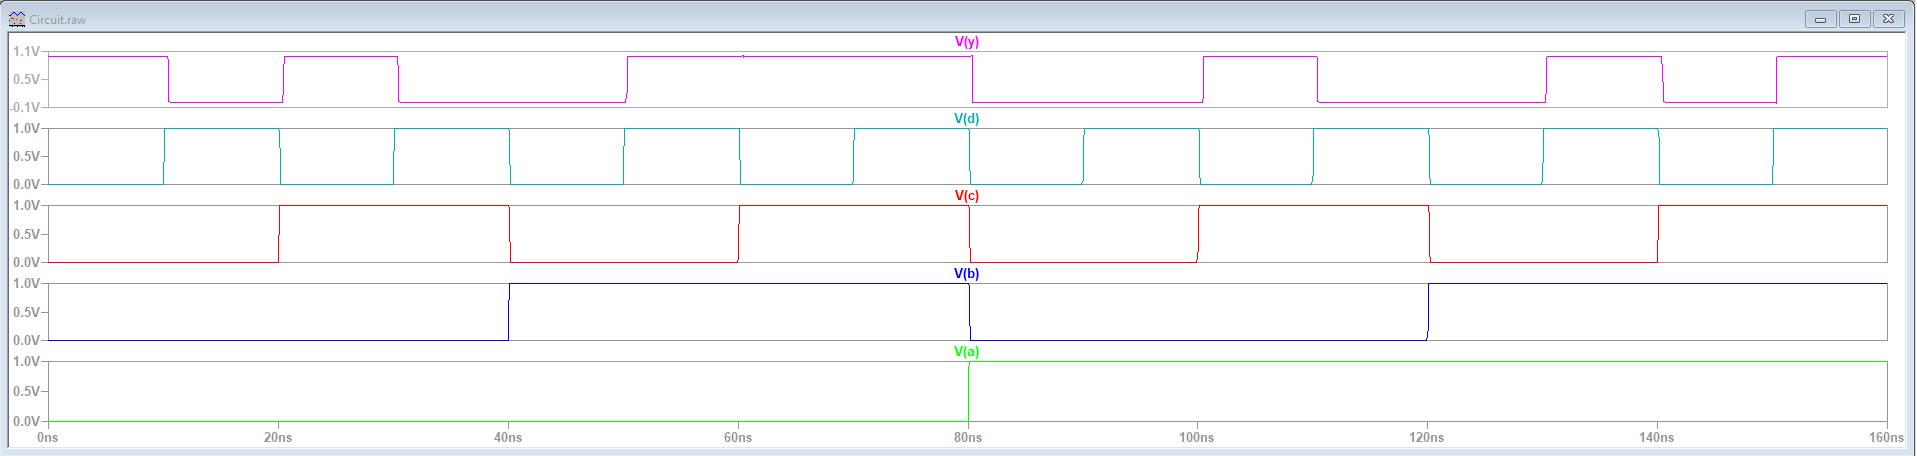
\includegraphics[width=\textwidth]{../pictures/simu.PNG}
            \caption{Simulation du circuit}
            \label{fig:simu}
        \end{figure}
    
    \subparagraph{}On remarque que toutes les 10 nano-secondes un état de la table de vérité est représenté. 
    On peut même y dessiner les états :
    
        \begin{figure}[H]
            \centering
            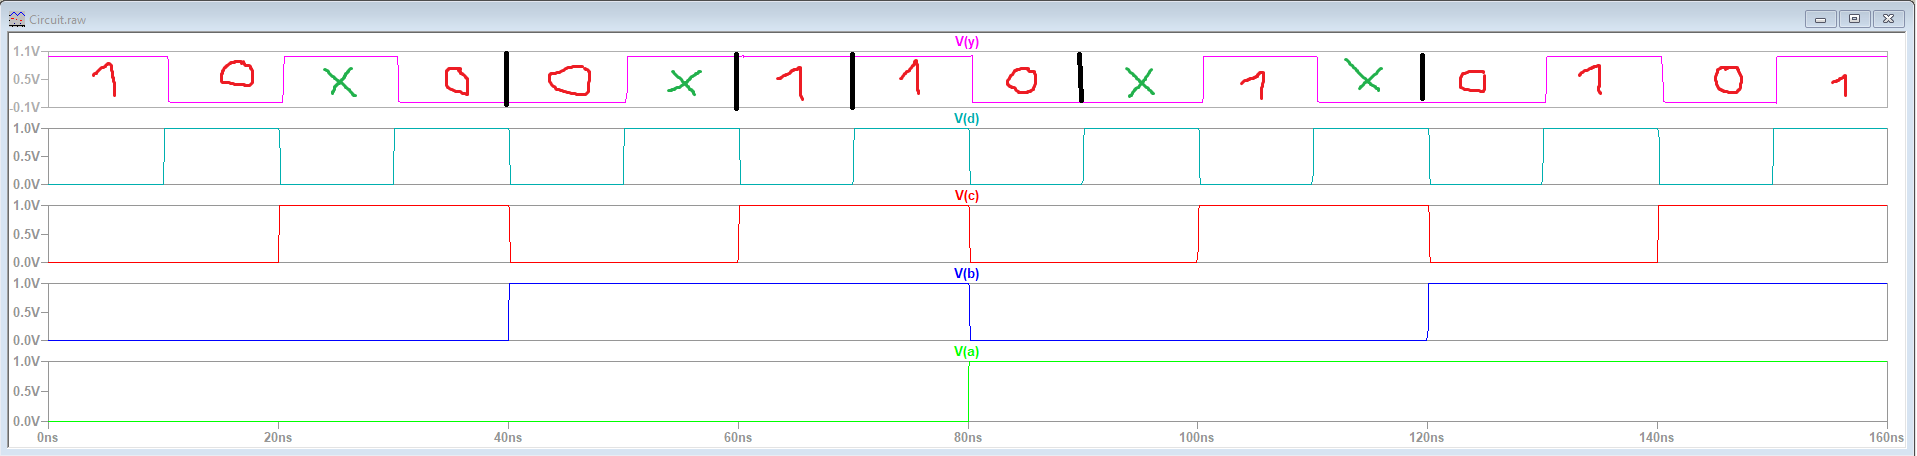
\includegraphics[width=\textwidth]{../pictures/simufun.PNG}
            \caption{Simulation du circuit avec les états de la table de vérité}
            \label{fig:simuT}
        \end{figure}



\section{Temps $t_{pd}$ et $t_{ccd}$}

    \subsection{Temps de contamination ($t_{ccd}$)}
    
        \subparagraph{}Le $t_{ccd}$ est le temps du chemin le plus court, c'est donc par conséquent le chemin qui passe
         par le produit $BD$, car il passe par une porte AND et deux portes OR mais pas par une porte NOT contrairement
          aux autres chemins. Par extraction de la simulation on obtient le graphe suivant : 
        
            \begin{figure}[H]
                \centering
                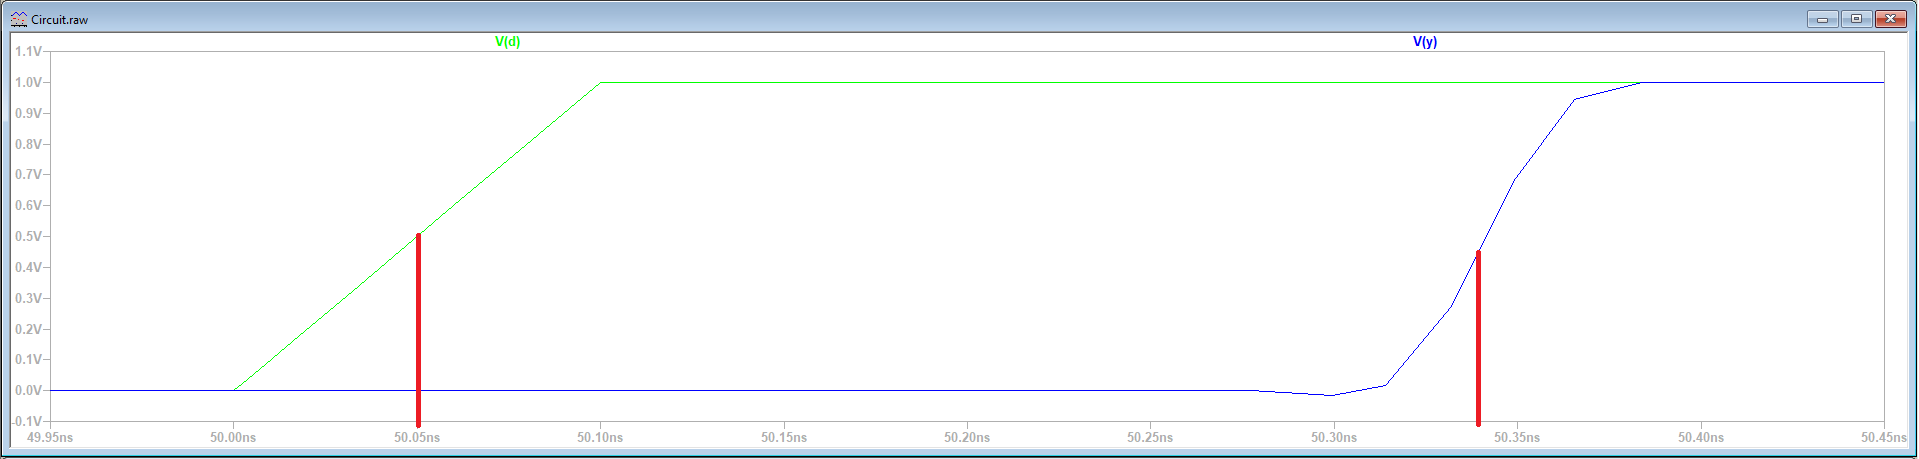
\includegraphics[width=\textwidth]{../pictures/contaminationT.png}
                \caption{Temps de contamination}
            \end{figure}
            
        \subparagraph{}On peut donc faire une approximation :
            
            \begin{align*}
                t_{ccd}\;&\approx\; 50,34\;ns - 50.5\;ns \\
                t_{ccd}\;&\approx\; 0,29\;ns
            \end{align*}
    
    \subsection{Temps de propagation ($t_{pd}$)}
        
        \subparagraph{}Le $t_{pd}$ est le temps du chemin le plus long, c'est donc par conséquent le chemin qui passe 
        par le produit $\overline{ABC}$, car chaque entrée passe par une porte NOT en plus d'un porte AND et deux 
        portes OR contrairement aux deux derniers chemins qui eux n'ont que 2 entrées passant par une porte NOT. Par 
        extraction de la simulation on obtient le graphe suivant :
        
            \begin{figure}[H]
                \centering
                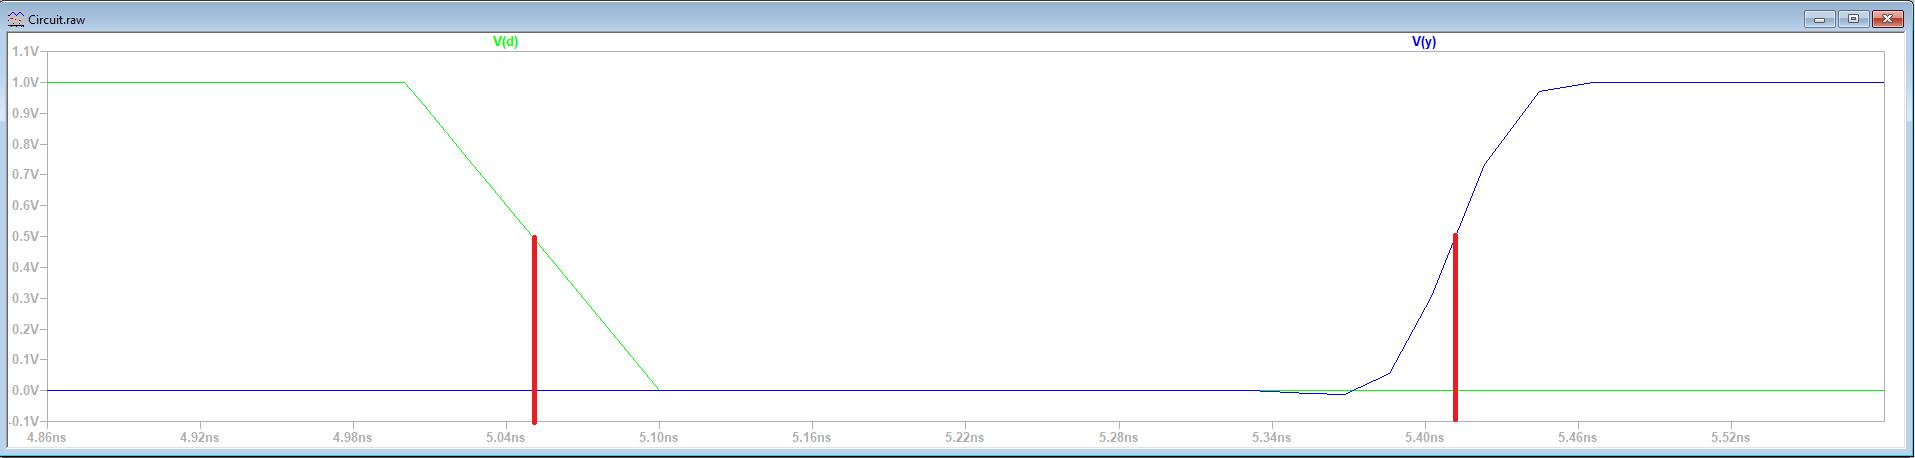
\includegraphics[width=\textwidth]{../pictures/propagationT.png}
                \caption{Temps de propagation}
            \end{figure}
            
        \subparagraph{}On peut donc faire une approximation :
        
            \begin{align*}
                t_{ccd}\;&\approx\; 5,41\;ns - 5,05\;ns \\
                t_{ccd}\;&\approx\; 0,36\;ns
            \end{align*}
        

\section{Conclusion}

    \subparagraph{}En conclusion, les résultats que j'ai obtenu sont en accord avec la simulation des 16 états de la 
    fonction logique. Ce travail permet de se rendre compte de la puissance du diagramme de Karnaugh pour optimiser
    une fonction logique à partir de sa table de vérité.

\end{document}